\documentclass[xcolor=svgnames]{beamer} 
\usefonttheme[onlymath]{serif}
\usepackage{tcolorbox}
\usepackage{multimedia}
\usepackage[utf8]{inputenc}
\usepackage[T1]{fontenc}
\usepackage[spanish]{babel}
\usepackage{mathtools}  % amsmath improved
%\usepackage{amsmath}
\usepackage{amssymb}
\usepackage{amsthm}
\usepackage{cancel}
\usepackage{multimedia}
\usepackage{algorithm2e}
%\usepackage{algorithm}
%\usepackage{algorithmic}
\usepackage{xcolor}
%\usepackage{pgfplots}
\usepackage{booktabs}   % Fancy table borders.

\newcommand{\grn}[1]{\textcolor{Green}{#1}}
\newcommand{\red}[1]{\textcolor{Red}{#1}}
\newcommand{\ple}[1]{\textcolor{Purple}{#1}}
\newcommand{\ong}[1]{\textcolor{DarkGoldenrod}{#1}}

%~~~~~~~~~~~~~~~~~~~~~~~~~~~~~~~~~~~~~~~~~~~~~~~~~~~~~~~~~~~~~~~~~~~~~~~~~~
%                         Beamer theme and colors

\usetheme{Warsaw}
%9 77 141

\definecolor{eafitColor}{rgb}{0.03515625,0.30078125,0.55078125}
\definecolor{eafitColor2}{rgb}{ 0.30859375,  0.5234375 ,  0.6953125}
\definecolor{mygreen}{rgb}{0.0 ,0.6, 0.0}


\usecolortheme[named=eafitColor]{structure} 
\setbeamercolor*{palette primary}{use=structure,fg=white,bg=eafitColor}
\setbeamercolor*{palette quaternary}{fg=white,bg=eafitColor2!90!eafitColor2}

%~~~~~~~~~~~~~~~~~~~~~~~~~~~~~~~~~~~~~~~~~~~~~~~~~~~~~~~~~~~~~~~~~~~~~~~~~~
%                    Put the page number on the slide

\defbeamertemplate*{footline}{shadow theme}
{%
  \leavevmode%
  \hbox{\begin{beamercolorbox}[wd=.5\paperwidth,ht=2.5ex,dp=1.125ex,leftskip=.3cm plus1fil,rightskip=.3cm]{author in head/foot}%
    \usebeamerfont{author in head/foot}\hfill\insertshortauthor
  \end{beamercolorbox}%
  \begin{beamercolorbox}[wd=.5\paperwidth,ht=2.5ex,dp=1.125ex,leftskip=.3cm,rightskip=.3cm plus1fil]{title in head/foot}%
    %\usebeamerfont{title in head/foot}\insertshorttitle\hfill\insertframenumber\,/\,\inserttotalframenumber%
    \usebeamerfont{title in head/foot}\insertshorttitle\hfill\insertframenumber\,/\,\inserttotalframenumber%
  \end{beamercolorbox}}%
  \vskip0pt%
}
%\setbeamertemplate{footline}{\hfill\insertframenumber/\inserttotalframenumber} 


%~~~~~~~~~~~~~~~~~~~~~~~~~~~~~~~~~~~~~~~~~~~~~~~~~~~~~~~~~~~~~~~~~~~~~~~~~~
%                             Color equations

\everymath{\color{blue}}
\everydisplay{\color{blue}}


\newcommand{\highlight}[1]{%
  \colorbox{yellow!50}{$\displaystyle#1$}}
  
\newcommand{\mathColor}[1]{{\color{blue}#1}}
\newcommand{\emphRed}[1]{{\color{red}#1}}

%~~~~~~~~~~~~~~~~~~~~~~~~~~~~~~~~~~~~~~~~~~~~~~~~~~~~~~~~~~~~~~~~~~~~~~~~~~
%                           Example environment

 \newtheoremstyle{example}{\topsep}{\topsep}%
     {}%         Body font
     {}%         Indent amount (empty = no indent, \parindent = para indent)
     {\bfseries}% Thm head font
     {}%        Punctuation after thm head
     {\newline}%     Space after thm head (\newline = linebreak)
     {\thmname{#1}\thmnumber{ #2}\thmnote{ #3}}%         Thm head spec

   \theoremstyle{example}
%   \newtheorem{example}{Example}[chapter]

%~~~~~~~~~~~~~~~~~~~~~~~~~~~~~~~~~~~~~~~~~~~~~~~~~~~~~~~~~~~~~~~~~~~~~~~~~~
%                           Vectors and Tensors

\if@mathematic
   \def\vec#1{\ensuremath{\mathchoice
                     {\mbox{\boldmath$\displaystyle\mathbf{#1}$}}
                     {\mbox{\boldmath$\textstyle\mathbf{#1}$}}
                     {\mbox{\boldmath$\scriptstyle\mathbf{#1}$}}
                     {\mbox{\boldmath$\scriptscriptstyle\mathbf{#1}$}}}}
\else
   \def\vec#1{\ensuremath{\mathchoice
                     {\mbox{\boldmath$\displaystyle#1$}}
                     {\mbox{\boldmath$\textstyle#1$}}
                     {\mbox{\boldmath$\scriptstyle#1$}}
                     {\mbox{\boldmath$\scriptscriptstyle#1$}}}}
\fi


\def\Real{\mathbb{R}}%
\newcommand{\mvM}{\text{max }\sigma_\text{vm} (\bs)}
\newcommand{\D}{\displaystyle}
\newcommand{\bm}[1]{\mbox{\boldmath$#1$}}

\def\bN{\bm{N}}
\def\bell{\boldsymbol \ell}%
\newcommand{\balpha}{\bm{\alpha}}
\def\bomega{\boldsymbol{\omega}}
\def\bsigma{\boldsymbol{\sigma}}
\DeclareMathOperator{\Div}{div}

\def\<{\left<}
\def\>{\right>}


% If you want to put an aditional slide with the section name at the beginning of 
% each section uncomment this two lines

%\AtBeginSection{\frame{\sectionpage}}
%\AtBeginSubsection{\frame{\subsectionpage}}

%~~~~~~~~~~~~~~~~~~~~~~~~~~~~~~~~~~~~~~~~~~~~~~~~~~~~~~~~~~~~~~~~~~~~~~~~~~~~~~~

\graphicspath{{../imagenes/},{figures2/}}

%\logo{Mecánica Aplicada\includegraphics[width=1.5cm]{logoEAFIT}\hspace{.5cm}} 
\logo{
\includegraphics[width=1.5cm]{../aux/LogoAzul.png}\vspace{-.2cm}} 
%  look later for this (manuel)
%http://tex.stackexchange.com/questions/27906/positioning-logo-in-the-front-page-as-well-as-slides

\title[ST0240-063]{Programación de Computadores }
\subtitle{Semana 1: Viernes 23 de Julio de 2016}
\author{
  Sergio Monsalve \\
  smonsal3@eafit.edu.co
}
\institute{
  Departamento de Informática y Sistemas \\
  Universidad EAFIT, Medellin, Colombia\\\vspace{0.5cm}
}
\date{Julio, 2016}

\makeatletter
    \newenvironment{withoutheadline}{
        \setbeamertemplate{headline}[default]
        \def\beamer@entrycode{\vspace*{-\headheight}}
    }{}
\makeatother

%~~~~~~~~~~~~~~~~~~~~~~~~~~~~~~~~~~~~~~~~~~~~~~~~~~~~~~~~~~~~~~~~~~~~~~~~~~
% Comment this line to remore the table of contents on top of the slide

%\setbeamertemplate{headline}{}

\beamertemplatenavigationsymbolsempty
%~~~~~~~~~~~~~~~~~~~~~~~~~~~~~~~~~~~~~~~~~~~~~~~~~~~~~~~~~~~~~~~~~~~~~~~~~~

\begin{document}

\setbeamertemplate{background canvas}{
%	    \includegraphics[width=1.1\textwidth]{region}
}
	
\begin{frame}[plain]
	\titlepage
\end{frame}
\setbeamertemplate{background canvas}{}
%\maketitle 

%~~~~~~~~~~~~~~~~~~~~~~~~~~~~~~~~~~~~~~~~~~~~~~~~~~~~~~~~~~~~~~~~~~~~~~~~~~

%\section*{Outline}
\begin{withoutheadline}
  \begin{frame}
    \setcounter{tocdepth}{1}
    \frametitle{Contenido}     
    \tableofcontents
  \end{frame}
\end{withoutheadline}

\section{Presentación}

\subsection{Docente}

\begin{frame}
  \frametitle{Docente}
  \begin{beamercolorbox}[wd=\textwidth,rounded=false,shadow=true]
    {block body example}
    \begin{centering}
    \begin{quote}
      Sergio Andrés Monsalve Castañeda \\
      Ingeniero de Sistemas\\
      Candidato a Master en Ingeniería Universidad EAFIT\\
      Oficina: Bloque 19 - 4 piso - 408\\
      Correo: smonsal3@eafit.edu.co %% \\
      %% Chat: fcardona@eafit.edu.co \\
      %% Twitter: @fcardonaeafit
    \end{quote}
    \end{centering}
  \end{beamercolorbox}
\end{frame}

\subsection{Libro guía}

\begin{frame}
  \frametitle{Libro guía}
  \begin{center}
      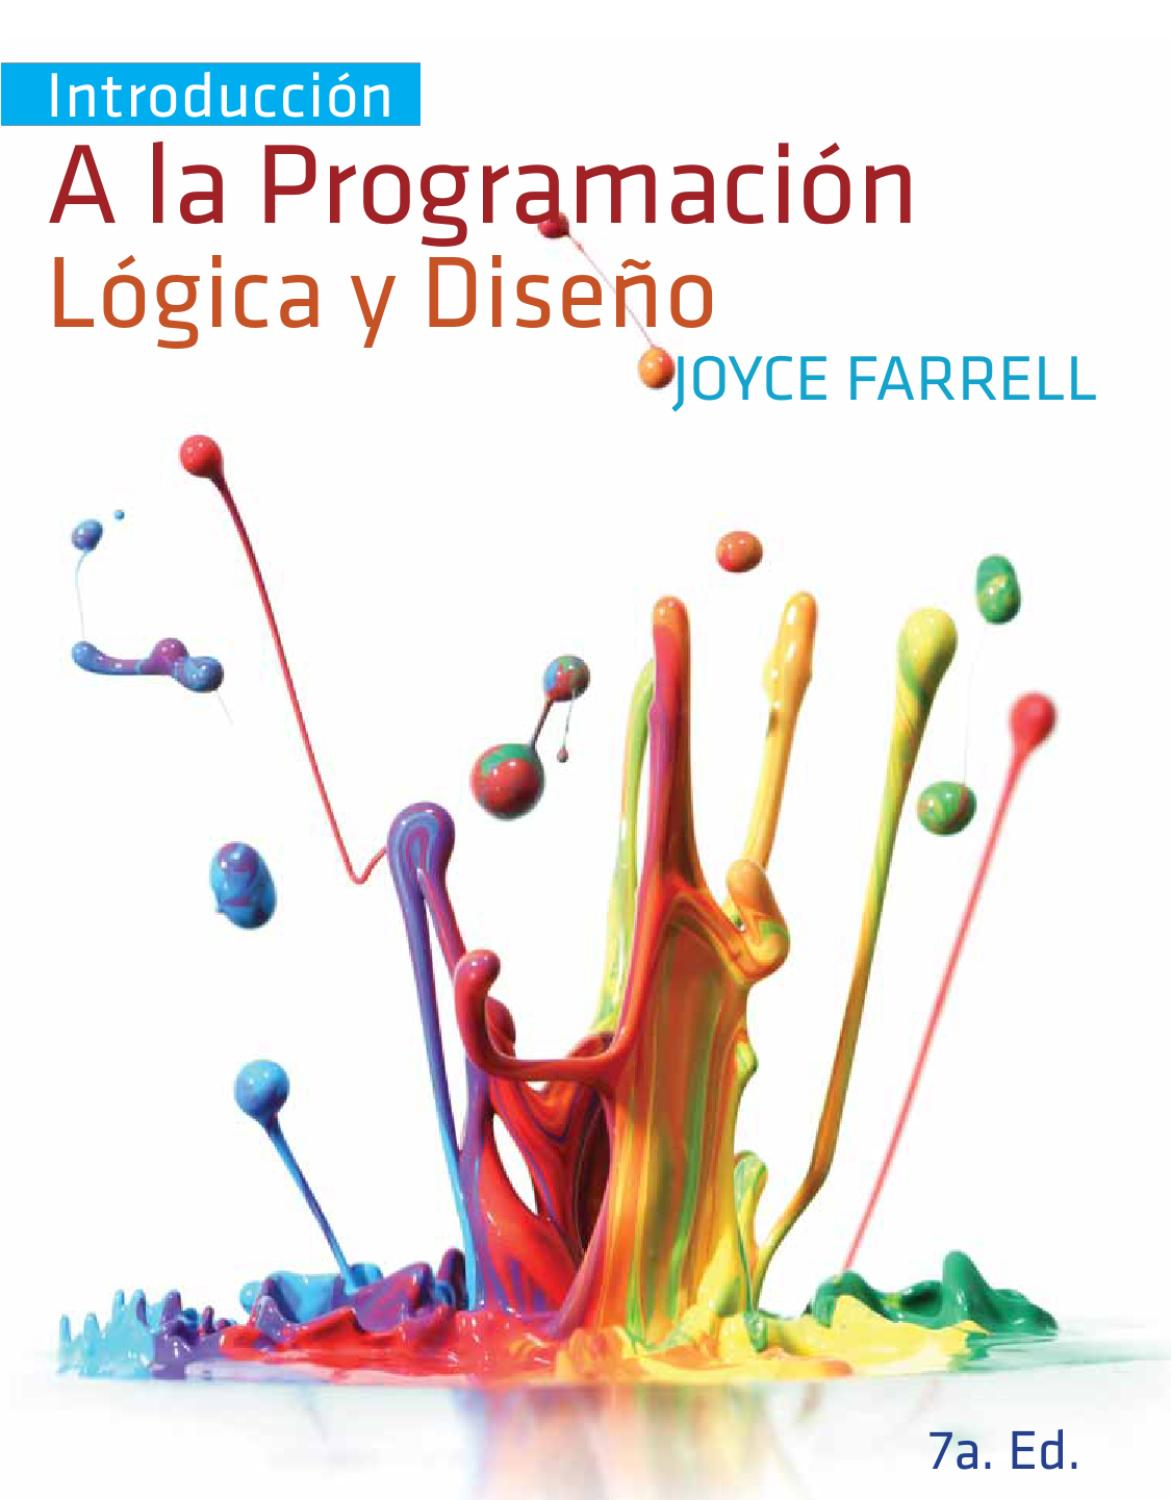
\includegraphics[width=0.38\textwidth]{../aux/farrell}\vspace{-.2cm}  \cite{farrell}
  \end{center}
  
\end{frame}

\subsection{Evaluación}

\begin{frame}
  \frametitle{Evaluación}
  \begin{itemize}%%[<+->]
  \item Seguimiento (10\%) 
  \item Taller 1 (5\%) - Semana 2  
  \item Taller 2 (5\%) - Semana 4  
  \item Taller 3 (10\%) - Semana 6 
  \item Taller 4 (10\%) - Semana 8 
  \item Taller 5 (10\%) - Semana 10
  \item Práctica 1 (15\%) - Semana 11
  \item Práctica 2 (15\%) - Semana 13
  \item Práctica Final (20\%) Semana 17
  \end{itemize}
\end{frame}

\subsection{Programa}

\begin{frame}
  \frametitle{Programa}
 \begin{tiny}
\begin{tabular}{|c|c|c|c|}
  \hline

  
Sem
& Fecha
& Contenido
&\begin{tabular}{c}
Actividad Evaluativa \\
 Actividad previa a Clase \\
 Actividad en Clase \\
 Actividad fuera de Clase\\
\end{tabular}
\\ \hline
1
& Julio 22
&

\begin{tabular}{c}
  
Computadores y lenguajes de programación \\
IDEs: Idle, PyCharm, Sublime, otros \\
Lenguajes Compilados vs Interpretados  \\
Tipos y variables  \\
Expresiones \\
Secuencias  \\
Entrada y Salida 1  \\
\end{tabular}
& Seguimiento (10\%)
\\ \hline
2
& Julio 29
& Funciones
Rangos
& Taller 1 (5\%)
\\ \hline
3
& Agosto 5
&

\begin{tabular}{c}
Ciclos\\
while, do-while, for, for.each \\
Condiciones (If,If-else, switch) \\  
\end{tabular}
&
\\ \hline
4
& Agosto 12
& Arreglos, Cadenas, Diccionarios, Listas
& Taller 2 (5\%)
\\ \hline
5
& Agosto 19
& Entrada y Salida 2
& 
\\ \hline
6
& Agosto 26
& Excepciones
& Taller 3 (10\%)
\\ \hline
7
& Septiembre 2
& Estructuras de Datos (Contenedores)
& 
\\ \hline

\end{tabular}
\end{tiny}
\end{frame}



\begin{frame}
  \frametitle{Programa}
   \framesubtitle{continuación}
 \begin{tiny}
\begin{tabular}{|c|c|c|c|}
  \hline



8
& Septiembre 9
& ordenamiento
& Taller 4 (10\%)
\\ \hline
9
& Septiembre 16
& Búsqueda
&
\\ \hline
10
& Septiembre 23
& Programación Orientada a Objetos
& Taller 5 (10\%)
\\ \hline
11
& Septiembre 30
& visualización de Información
& 
\\ \hline
12
& Octubre 7
&(DIAS EAFIT)
& 
\\ \hline
13
& Octubre 14
& Matlab
& PRACTICA 1(15\%)
\\ \hline
14
& Octubre 21
& Matlab
& 
\\ \hline
15
& Octubre 28
& Visual Basic for Applications VBA(excel)
& PRACTICA 2 (15\%)
\\ \hline
16
& Noviembre 4
& Programación Orientada a Objetos
& 
\\ \hline
17
& Noviembre 11
& Colchon
& PRÁCTICA FINAL (20\%)
\\ \hline
\end{tabular}
\end{tiny}
\end{frame}


\section{Introducción}


\subsection{Historia}

\subsection{IDE}

\begin{frame}
  \frametitle{IDE's}
  \begin{itemize}
    \item Idle
    \item Sublime Text
    \item Pycharm
    \item otros
  \end{itemize}
\end{frame}

\begin{frame}
  \frametitle{Pycharm}
  \begin{itemize}
    \item Idle
    \item Sublime Text
    \item Pycharm
    \item otros
  \end{itemize}
\end{frame}

\subsection{Python}


\begin{frame}
  \frametitle{}
  \begin{itemize}
    \item Tipos
    \item Variables
    \item Entrada
    \item Salida
  \end{itemize}
\end{frame}





\section{Conclusiones}

\begin{frame}
  \frametitle{Pendientes para la próxima clase}
  \begin{itemize}
  \item{Libro guia: Capitulos 1 y 2}
    \item{SPOJ: problema de Prueba}
  \item{Quiz 1\%}
  \item{Taller 6\%}
  \end{itemize}
\end{frame}


\subsection{Referencias}

\begin{thebibliography}{9}
\bibitem{farrell}
  Joyce Farrell,
 \emph{Introducción a la programación: lógica y diseño},
  Thomson Learning,
  2001.
 
\end{thebibliography}


\end{document}
